\documentclass[]{rsos}%%%%where rsos is the template name

\usepackage{amsmath,amsfonts,amssymb}
\usepackage[english]{babel}
\usepackage[latin1]{inputenc}
\usepackage[T1]{fontenc}
\usepackage{color}
\usepackage{float}
\usepackage{verbatim}
\usepackage{graphicx}
\usepackage{bm}
\usepackage{mathtools}
\usepackage{stmaryrd}
\usepackage{anyfontsize}
\usepackage{color}
\usepackage{subcaption}
% \usepackage{subfigure}


%%%% *** Do not adjust lengths that control margins, column widths, etc. ***

%%%%%%%%%%% Defining Enunciations  %%%%%%%%%%%
\newtheorem{theorem}{\bf Theorem}[section]
\newtheorem{condition}{\bf Condition}[section]
\newtheorem{corollary}{\bf Corollary}[section]
%%%%%%%%%%%%%%%%%%%%%%%%%%%%%%%%%%%%%%%%%%%%%%%


\begin{document}

%%%% Article title to be placed here
\title{Supplemental Materials: On the dynamics of starvation, mortality, and the ephemeral nature of mammalian megafauna}

\author{%%%% Author details
Taran Rallings$^{1}$, Christopher P Kempes$^{2}$, Justin D. Yeakel$^{1}$} 
% and X. Third author$^{3}$}%

%%%%%%%%% Insert author address here
\address{
$^{1}$School of Natural Sciences, University of California Merced\\
$^{2}$Santa Fe Institute}
% $^{2}$Second author address\\
% $^{3}$Third author address}

%%%% Subject entries to be placed here %%%%
\subject{foodwebs, paleontology, ecology}
%%%% Keyword entries to be placed here %%%%
\keywords{foodwebs, mammals, foraging}

%%%% Insert corresponding author and its email address}
\corres{Taran Rallings\\
\email{trallings@ucmerced.edu}}

% %%%% Abstract text to be placed here %%%%%%%%%%%%
% \begin{abstract}
% Main Takeaway points

% 1) The mass-density relationship represented by Damuth's Law can be approximated with a 2D allometric consumer-resource model that includes starvation dynamics.

% 2) The magnitude of consumer population density is set by the environmental context of resource growth rates and carrying capacity interacting with fixed internal resource use. The nature/slope of the mass-density relationship in Damuth's Law is set by internal processes of reproduction and resource use regardless of environmental context. 

% 3) Increases in actuarial mortality rates can radically alter consumer community structure and lead to the exclusion of small-bodied consumers despite having a stronger overall impact on large bodied consumers.  

% 4) Predation is very cool. 

% 5) The harvest of consumer populations lowers the maximum body mass of species in a consumer community if the rate of harvest does not decrease with consumer mass. 

% \end{abstract}
% %%%%%%%%%%%%%%%%%%%%%%%%%%%


\maketitle

\renewcommand{\thepage}{S\arabic{page}}
\renewcommand{\thesection}{S\arabic{section}}
\renewcommand{\thetable}{S\arabic{table}}
\renewcommand{\thefigure}{S\arabic{figure}}
\renewcommand{\figurename}{Figure}
\setcounter{figure}{0}


\subsection{Dimensional system to non-dimensionalized system}

Recall that $\hat{k} = k/2$ where $k$ is the resource carrying capacity.
We begin with the dimensional consumer-resource system
\begin{align}
    \frac{dC_d}{dt} &= \lambda_{\rm C}\frac{R_d}{\hat{k}}C_d- \sigma \left(1 - \frac{R_d}{k} \right)C_d, \nonumber \\ 
    \frac{dR_d}{dt} &= \alpha R_d \left(1 - \frac{R_d}{k} \right) - \left(\frac{\lambda^{\rm max}_{\rm C}}{Y_{\rm C}}R_d + \rho \right)C_d.
    \label{eq:2dDD1}
\end{align}
We define dimensionless variables $C = fC_d$, $R = qR_d$, and $t = st_d$, giving us
\begin{align}
    \frac{dC}{dt} &= \frac{1}{s}\left[\lambda_{\rm C}\frac{R}{q\hat{k}}C- \sigma \left(1 - \frac{R}{qk} \right)C\right], \nonumber \\ 
    \frac{dR}{dt} &= \frac{1}{s}\left[\alpha R \left(1 - \frac{R}{qk} \right) - \left(\frac{\lambda_{\rm C}}{Y_{\rm C}\hat{k}q}R + \rho \right)C\right].
    \label{eq:2dDD2}
\end{align}
We then set $s=1$, $q = 1/k$, and $f = 1/Y_C\hat{k}$ to get
\begin{align}
    \frac{dC}{dt} &= \lambda_{\rm C}\frac{R}{\hat{k}/k}C- \sigma \left(1 - R \right)C, \nonumber \\ 
    \frac{dR}{dt} &= \alpha R \left(1 - R \right) - \left(\lambda_{\rm C}R_d + \frac{\rho Y_C \hat{k}}{k} \right)C.
    \label{eq:2dDD3}
\end{align}
We then define the dimensionless parameters $\xi = k/\hat{k}$ and $\delta = \rho Y_C \hat{k}/k$ to get 
\begin{align}
    \frac{dC}{dt} &= \xi \lambda_{\rm C}R C- \sigma \left(1 - R \right)C, \nonumber \\ 
    \frac{dR}{dt} &= \alpha R \left(1 - R \right) - \left(\lambda_{\rm C}R_d + \delta \right)C.
    \label{eq:2dDD4}
\end{align}

\subsection{Derivation of allometric vital rates}


%  include detailed parameter stuff and derivations

% - explain the foundation of the 3D model from the starvation paper

% - explain the collapse to 2D, how it was done and why it works

% - explain, in detail, where on earth all of these parameters come from

% - explain the role of resource carrying capacity in the consumer dynamics

% - justify under what conditions the k thing makes sense and where it doesn’t

% - explain the methods of analysis – analytical, simulation, and population dynamics

% - explain how the relationship between parameters and real resources/herbivores was done

% - explain how the new starvation mortality works

\subsection{The influence of variations in model parameters and allometric rates}


While our framework dictates that plant growth rates and carrying capacities are directly proportional to consumer steady states, we can gain insight into what drives the very large range of observed consumer densities by exploring the observed ranges of $\alpha$ and $k$ in terrestrial systems.
We assume an intrinsic growth rate roughly that of grass where $\alpha = 9.45\times 10^{-9}$ (s${}^{-1}$; REF), whereas observations among terrestrial plants reveal a range in growth rates from $2.81\times 10^{-10}$ to $2.19\times 10^{-8}$ \cite{michaletz2014convergence}, according with a change in $\alpha$ of roughly 97\% lower and 130\% higher than the set value. 
By incorporating this range into our the estimated resource growth rate, we observe that we can account for a large portion of consumer steady state densities around the mean density given by Eq. \ref{eq:2d} (inner shaded region, Fig. \ref{fig:2ddensities}).
If we additionally adjust the carrying capacity $k$ of the resource to 90\% less-than and 150\% more-than the assumed value of $23\times 10^3$ g/m${}^2$, our framework accounts for nearly the full range of mammalian steady state densities (outer shaded region, Fig. \ref{fig:2ddensities}).
In this context, the upper-boundary of $k$ observed to capture most higher herbivore densities is ca. 34 kg/m${}^2$, which is on the higher end of estimated live above-ground biomass densities in terrestrial forests such as in Isle Royal and the Allegheny National Forest \cite{de2017simulating}.
% With an energy density of ca. 5.77 kiloJoules/gram, higher than but within range of the carrying capacity of $664\times10^3$ kJ/m${}^2$, [within the range of possibility for terrestrial systems, REF].


%Variations in steepness of slope
Our model's ability to capture the bounds of mammalian densities at low and high productivity invites some speculation into the actual steepness of the mass-density relationship.
While the best-fit slope to Damuth's Law is -0.77 (-0.74 using XX) we also observe that the steeper relationship given by our framework better captures the boundaries of mass-density data, whereas varying the intercept of the statistical best-fit would not capture the lower-density outer-boundary of larger species. % - especially those between $10^4$ and $10^5$ grams.
While within-clade mass-density relationships often reveal a shallower slope than if measured across clades \cite{Pedersen:2017he}, it is possible that the absence of data for larger mammals may bias estimates of the slope towards smaller (shallower) values.
Mammalian communities have undergone significant anthropogenic restructuring throughout the Holocene (REF), such that many larger species are excluded from the mass-density relationship by way of extinction (REF), and the greater prevalence of smaller species may introduce size-dependent biases.
For example, if species $<100$ g are excluded, the empirical mass-density slope steepens from $-0.77$ to $-0.85$.
% Because of the extinction-related bias of contemporary mammalian faunas (REF), the over-representation and influence of extant size classes should be considered when evaluating macroecological relationships (REF). 

Considering how variations to the underlying energetic parameters driving consumer-resource dynamics alters the expected mass-density relationship may shed light on key constraints shaping mammalian communities. 
% PARAMETERS INFLUENCING INTERCEPT ONLY
We next explore how variations in the vital rates included in the consumer-resource model modify the expected intercept and slope of the mammalian mass-density relationship.
Different vital rates impact the mass-density relationship in three distinct ways, by either \emph{i}) influencing only the mass-density slope, \emph{ii}) influencing only the mass-density intercept, or \emph{iii}) influencing both.
Aside from the resource growth rate and carrying capacity, our framework also includes the intrinsic consumer reproductive rate $\lambda^{\rm max}_C$, the consumer yield coefficient $Y_C$, and the maximum rate of starvation $\sigma$.
We introduce changes to these rates as, for example, $\lambda^{\rm max\prime}_C = \lambda^{\rm max}_C(1+\chi)$, where $\chi \in (-1,2)$ represents the proportion increase or decrease of the altered parameter denoted by ${}^\prime$.
We note that the recovery rate $\rho$ is sufficiently small that alterations do not have an influence on either the consumer mass-density intercept or slope.


Importantly, changes to the starvation rate have a large effect on both the consumer-density intercept and slope (Fig. \ref{fig:corr}E,F).
We observe that decreasing $\sigma$ from the expected value ($\chi<0$) serves to increase the steady state intercept, while decreasing the mass-density slope.
By comparison, increasing $\sigma$ from the expected value ($\chi>0$) has less effect on the mass-density relationship.
In the consumer-resource model described in Eq. \ref{eq:2d}, starvation is the sole source of consumer mortality, and therefore plays an out-sized role in determining consumer steady states. 
As this mortality is reduced, consumer densities increase, raising the intercept.
However, as consumer starvation rates decline we observe a steeper mass-density slope.
Reduced starvation rates therefore principally benefit the steady state densities of smaller species, with reduced effects observed for larger-bodied mammals.
Because fat biomass scales super-linearly with body mass (see methods; REFS), the populations of larger consumers are more resilient to the effects of starvation, whereas those of smaller consumers are more prone.

% Changes to the starvation rate have a large effect on both the consumer-density intercept and slope (Fig. \ref{fig:corr}E,F).
% We observe that decreasing $\sigma$ from the expected value ($\chi<0$) serves to increase the steady state intercept, while decreasing the mass-density slope.
% By comparison, increasing $\sigma$ from the expected value ($\chi>0$) has less effect on the mass-density relationship.
% In the consumer-resource model described in Eq. \ref{eq:2d}, starvation is the sole source of consumer mortality, and therefore plays an out-sized role in determining consumer steady states. 
% As this mortality is reduced, consumer densities increase, raising the intercept.
% However, as consumer starvation rates decline we observe a steeper mass-density slope.
% Reduced starvation rates therefore principally benefit the steady state densities of smaller species, with reduced effects observed for larger-bodied mammals.
% Because fat biomass scales super-linearly with body mass (see methods; REFS), the populations of larger consumers are more resilient to the effects of starvation, whereas those of smaller consumers are more prone.



% PARAMETERS INFLUENCING SLOPE ONLY
The consumer's maximal rate of reproduction $\lambda^{\rm max}_C$ influences only the mass-density slope except for the case $\chi \rightarrow -1$, where growth becomes zero.
Above this trivial limit, we observe the consumer growth rate to have a negative effect on the mass-density slope, such that as the growth rate increases, the mass-density relationship becomes steeper (Fig. \ref{fig:corr}A,B).
As the intercept does not change, this means that the steady states of larger bodied consumers decline with increasing $\lambda_C^{\rm max}$, while those of smaller-bodied consumers remain unaltered, though the effect is slight.
% Because larger organisms more efficiently convert resource to 
% , though this effect is nearly imperceptible and not of sufficient magnitude to change the mass-density relationship.
Of more interest is the effect of the yield coefficient $Y_C$ and starvation rate $\sigma$ (Fig. \ref{fig:corr}C-F).
The yield coefficient represents the conversion of resources to consumer biomass, where an increase in $\chi$ correlates to large increases in consumer steady state without altering the mass-density slope. 
Here we observe that increased efficiency in converting resource to consumer biomass will have an effect similar to increasing resource productivity, as the effective abundance of the resource is greater when relatively fewer resources fuel a given unit of consumer biomass.
Because $Y_C \propto E_d$ where $E_d$ is the energy density of the resource (see methods), resource quality is therefore expected to translate directly to higher consumer steady state densities.

\subsection{Derivation of allometric natural mortality}
% - explain how the new survivorship mortality works

\subsection{Derivation of allometric capture rates}
% - explain how the new predation mortality works

% \begin{align}
% \frac{\rm d}{\rm dt}C &= -bP^*C, \nonumber \\
% 	b &= \frac{\lambda_{\rm P}}{Y_P k_C^{\rm max}},
% \end{align}
% where $b$ is the capture efficiency of the predator on the consumer, $P^*$ is the steady state density of the predator population, $\lambda_P$ is the maximum growth rate of the predator, $k_C^{\rm max}$ is the density of the consumer population that maximizes this predator growth, and $Y_P$ is the yield coefficent for the predator.
% As we are not tracking ${\rm d}P/{\rm dt}$, we assume a constant predator population density given by Damuth's Law, but where the slope and intercept consider only measured densities of predatory mammals.
% If $P$ is g/m${}^2$, the density of individuals/m${}^2$ then follows $(1/M_P)P^*(M_P) \propto M_P^{-0.88}$. 


% The predator's yield $Y_P$ is calculated
% \begin{equation}
% Y_P = \frac{M_P E_C}{\int_0^{t_{\lambda_P}}B_0^Pm_P(t)^\eta {\rm dt}},
% \end{equation}
% where $m_P(t)$ is the ontogenetic mass of an individual predator as it grows over time to an adult mass $M_P$.
% The parameters $t_{\lambda_P}$ and $B_0^P$ are the timescale associated with reaching reproductive maturity and the metabolic coefficient for predatory mammals, respectively, and $\eta=-3/4$ is the metabolic exponent.
% In words, the predator yield scales proportionally with the individual mass of the predator (g) and the energy density of prey $E_C$ (J/g), normalized to the lifetime energetic needs of a predator reaching maturity (J).
% Accordingly, the predator yield coefficient describes the grams of predator produced per gram of prey consumed.

% We assume that predators consume all non-skeletal mass of prey. 
% Because the amount of consumable tissues with different energy densities within an herbivore varies allometrically, so too should the energy density $E_C$.
% We consider four primary tissue groups: a consumable set composed of muscle, fat, and \emph{other} tissues, and an non-consumable set composed only of skeletal tissues.
% If the scalings associated with fat, muscle, and skeletal tissues are $M_C^{\rm fat}=f_0 M_C^{1.19}$, $M_C^{\rm musc} = g_0 M_C^{1.00}$, and $M_C^{\rm skel} = h_0 M_C^{1.09}$, the scaling of the \emph{other} tissue (gut tissue, organ tissue, etc) is given by $M_C^{\rm other} = M_C - (M_C^{\rm fat} + M_C^{\rm musc} + M_C^{\rm skel})$.
% The energy density of fat is $E_{\rm fat} = 37700$ J/g, whereas the energy density of muscle is $E_{\rm musc} = 17900$ J/g.
% If we assume that gut and organ tissues have roughly the same energy density as muscle, the attainable energy density for an herbivore of size $M_C$ is given by
% \begin{equation}
% 	E_C(M_C) = E_{\rm fat}\frac{M_C^{\rm fat}}{M_C} + E_{\rm musc}\left(\frac{M_C^{\rm musc}}{M_C} + \frac{M_C^{\rm other}}{M_C} \right).
% \end{equation}

% Another important consideration is that we have assigned $k_C^{\rm max}$ to represent the consumer density maximizing predator growth $\lambda_P$.
% Because predator growth is proportional to prey growth, and prey growth is responding to a logistically growing resource $R$, we assume that predator growth is maximized when prey growth is maximized, which occurs when the resource reaches its half-saturation point $R = k_R/2$ g/m${}^2$, where we assume $k_R = 23000$ g/m${}^2$.
% The translated available consumer biomass represented by this half-saturation point is then given by $k_C^{\rm max} = Y_C k_R/2$ (consumer g/m${}^2$) where $Y_C$ is the consumer yield coefficient, giving the grams of consumer per grams of resource and calculated analagously to $Y_P$, such that
% \begin{equation}
% 	Y_C = \frac{M_C E_R}{\int_0^{t_{\lambda_C}}B_0^C m_C(t)^\eta {\rm dt}},
% \end{equation}
% where $m_C(t)$ is the ontogenetic mass of an individual herbivorous consumer as it grows over time to an adult mass $M_C$.
% The parameters $t_{\lambda_C}$ and $B_0^C$ are the timescale associated with reaching reproductive maturity and the metabolic coefficient for herbivorous mammals, respectively, and $\eta=-3/4$ is the metabolic exponent.
% Moreover, we assume a resource energy density that approximates graze, such that $E_R = 18200$ J/g.

% Because predator-prey relationships tend to be determined largely by the body sizes of predator and prey, the mortality of a prey consumer due to predation requires us to assume a consumer with mass $M_C$ has a predator with body mass $M_P$.
% The probability of a trophic interaction between predators and prey $\ell_{C,P}$ as a function of the body sizes of both follows a logit relationship, where
% \begin{equation}
% 	\log \left(\frac{Pr(\ell_{C,P})=1}{Pr(\ell_{C,P})=0}\right) = q_0 + q_1 \log \left(\frac{M_C}{M_P}\right) + q_2 \log^2\left(\frac{M_C}{M_P}\right).
% \end{equation}
% and the parameters ${\bm q} = (q_0,q_1,q_2)$ are fitted to an adjacency matrix describing empirical interactions between predators and prey of different body sizes within a community. 
% The result for diverse terrestrial mammalian communities such as that in the Serengeti results in a Guassian-shaped distribution in log body mass space, where for a particular predator mass there is a range of prey masses for which the linking probability is high, and below or above which the linking probability is low.
% We describe this peak of this linking probability as the optimal prey size for a particular predator, which can be algebraically manipulated to provide the optimal predator size associated with a particular consumer prey, such that
% \begin{equation}
% 	M_P^{\rm opt} = M_C {\rm e}^{\frac{q_1}{2 q_2}}.
% 	\label{eq:opt}
% \end{equation}
% Given best-fits of ${\bm q}$ for interactions in the Serengeti, one of the few remaining diverse terrestrial mammalian communities, we observe that $\log (M_P^{\rm opt}) < \log(M_C)$, meaning that predators are smaller than their prey.
% We note that in aquatic systems the reverse relationship is observed, given those predators tend to be gape-limited.
% If we operate under the assumption that - on average - a consumer with mass $M_C$ will suffer mortality by a predator with mass $M_P^{\rm opt}$, we obtain a mortality rate $-bP^*$ that varies only as a function of consumer mass $M_C$.


\subsection{Derivation of harvesting mortality}
% - explain how the new harvesting mortality works

\clearpage
% \subsection{Supplementary Figures}



\begin{figure}
  \centering
% \begin{subfigure}
\includegraphics[width=0.45\textwidth]{fig_intmod.pdf}
% \end{subfigure}
% \begin{subfigure}
% \includegraphics[width=0.45\textwidth]{fig_slopemod.pdf}
% \includegraphics[width=0.9\textwidth]{starvation_reproductionrates.png}
% \end{subfigure}
\caption{The effects of changes to metabolic parameters on the prediction of the mass-density relationship.}
\label{fig:corr1}
\end{figure}

\begin{figure}
  \centering
  % \begin{subfigure}
  % \includegraphics[width=0.45\textwidth]{fig_intmod.pdf}
  % \end{subfigure}
  % \begin{subfigure}
  \includegraphics[width=0.45\textwidth]{fig_slopemod.pdf}
  % \includegraphics[width=0.9\textwidth]{starvation_reproductionrates.png}
  % \end{subfigure}
  \caption{The effects of changes to metabolic parameters on the prediction of the mass-density relationship.}
  \label{fig:corr2}
\end{figure}
  


\begin{figure*}
  \centering
  \includegraphics[width=0.6\textwidth]{fig_meanpredsize34_log.pdf}
  \caption{
	 Expected predator masses for contemporary large-bodied ($>10^5$ g) terrestrial predators and prey. 
	 Expected predator sizes as a function of herbivore size class were determined by reconstructing dietary samples from observed trophic interactions for cheetah, wild dogs, dholes, leopards, hyenas, lions, and tigers from \cite{Hayward2008} (REF others), where masses for both predators and prey were allowed to vary $\pm 20\%$ from measured estimates.
	 The blue line denotes the best fit relationship, given by ${\rm E}(M_P|M_C) = p_0 M_C^{p_1}$, where $p_0 = 11786.8$ g and $p_1 = 0.194$.
	 The red line represents a modified PPMR where $p_0^\prime = p_0(1+\chi_{\rm int})$ and $p_1^\prime = p_1(1+\chi_{\rm slope})$ where $\chi_{\rm int} = 0.97$ and $\chi_{\rm slope} = 1.50$ that allows megatrophic interactions and resides within the white band displayed in Fig. \ref{fig:predrate}C,D.
	 This relationship is entirely hypothetical, but does not stray far from observations of contemporary species, describes megapredators that predate on megaherbivores, and results in threshold herbivore and carnivore size classes that permit dynamically feasible megatrophic interactions.
	 The black line denotes the 1:1 line.
  }
  \label{fig:ppmr}
\end{figure*}

\begin{figure*}
  \centering
  \includegraphics[width=0.6\textwidth]{fig_maxpreyvar.pdf}
  \caption{
	  The effect of changing the reliance of predator growth $f$ on the single herbivore consumer population. If $f=1$, the predator solely relies on the herbivore consumer. If $0<f<1$, the predator relies on the herbivore population to support a fraction of its growth. If $f>1$, the predator is removing more biomass than is necessary to support its growth.
	  Blue region denotes herbivore threshold mass range characterizing $f=1 \pm 0.1$.
	  Yellow line denotes the mass range of contemporary elephants.
	  Vertical dashed line denotes the size of the largest terrestrial mammal (Deinotherium at ca. $1.74\times 10^7$, corresponding to $f=0.37$, such that a predator is supporting a little more than 1/3 of its growth from the herbivore consumer.
  }
  \label{fig:maxpreyvar}
\end{figure*}

\begin{figure*}
  \centering
  \includegraphics[width=0.6\textwidth]{fig_megamammal.pdf}
  \caption{
    Mass ranges corresponding to feasible megatrophic interactions (where herbivore and predator threshold masses are $> 6\times10^5$ g) across variations to the assumed predator-prey mass ratio (PPMR), demarcated by the white bands in Fig. \ref{fig:predrate}C,D, and under the assumption specialist predation ($f=1$). 
% 	  The range of herbivore and carnivore threshold size classes where both species are characterized by mega- body mass ($>6\times10^5$ g) under the condition of predator specialization and across variable PPMRs, where ${\rm E}(M_P|M_C) = p_0(1+\chi_{\rm int}) M_C^{p_1(1+\chi_{\rm slope})}$ and both $\chi_{\rm int}$ and $\chi_{\rm slope} \in (-0.99,2)$.
  }
  \label{fig:megamammal}
\end{figure*}

\begin{figure*}
  \centering
  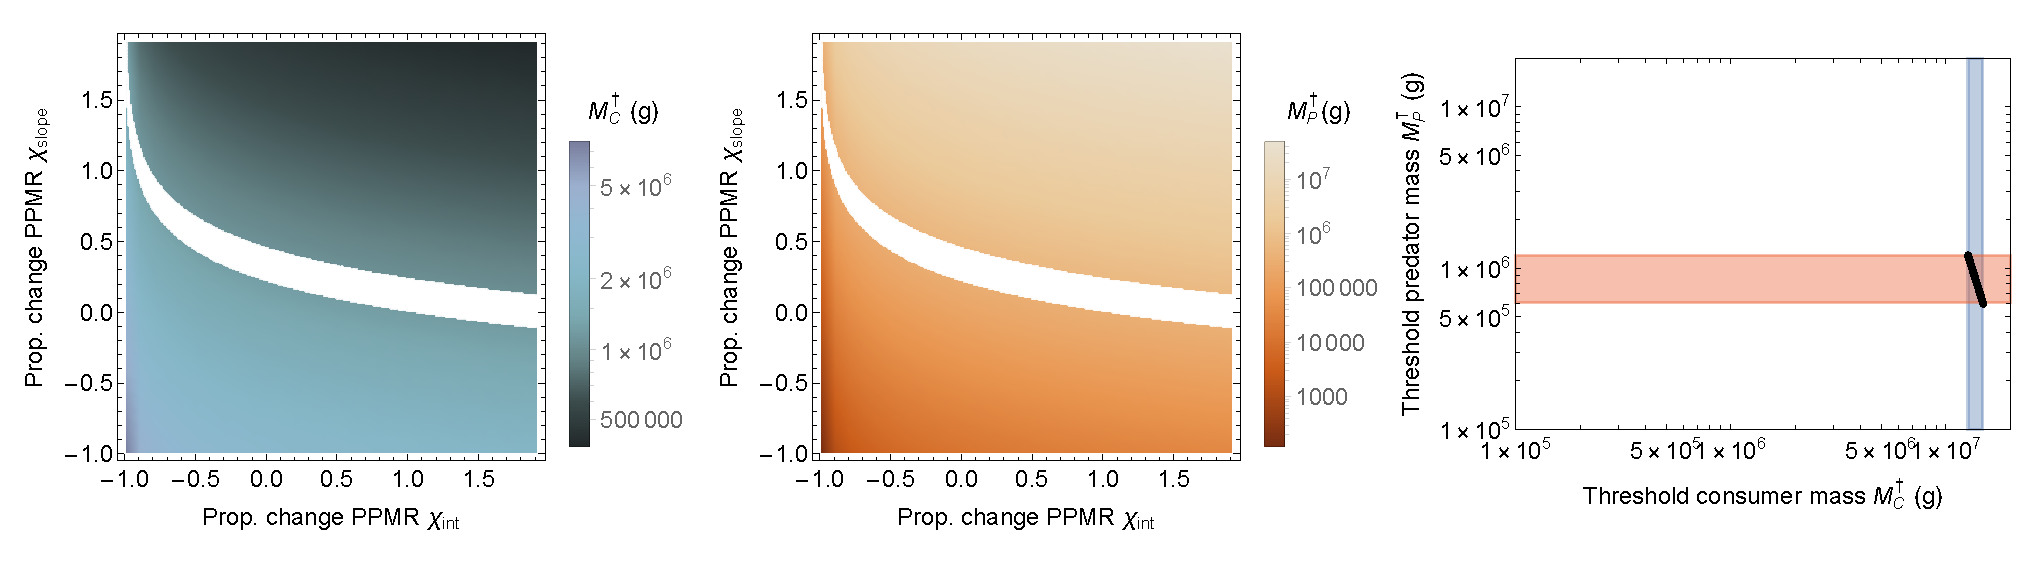
\includegraphics[width=1\textwidth]{fig_megamammal_generalist.png}
  \caption{
    The effects of predator generalization on A) threshold herbivore mass $M_C^\dagger$ and B) threshold predator mass $M_P^\dagger$ across variable PPMRs, where ${\rm E}(M_P|M_C) = p_0(1+\chi_{\rm int}) M_C^{p_1(1+\chi_{\rm slope})}$ and both $\chi_{\rm int}$ and $\chi_{\rm slope} \in (-0.99,2)$.
    White bands denote regions of $\chi_{\rm int}$ and $\chi_{\rm slope}$ where megatrophic interactions are feasible (both perdator and herbivore threshold masses are $> 6\times10^5$ g).
    C) Mass ranges corresponding to feasible megatrophic interactions in the white bands in A and B.
  }
  \label{fig:megamammalgen}
\end{figure*}

\begin{figure*}
  \centering
\includegraphics[width=0.9\textwidth]{harvest_scaling_plot.png}
\caption{
  }
  \label{fig:harvestscaling}
\end{figure*}

\clearpage

% \vspace{0.5cm}

% \emph{Explain the basic parameters of the model}

% $\lambda$ is the maximum consumer reproduction rate (1/s) under ideal resource conditions. Structurally, its form is ln(2)/Tlam. The fecundity of the consumer is given by the logged number in the numerator, 2 in this case. Tlam is the time from reproductive event to maturity for an organism of a given bodymass. 


% $\mu$ is the survivorship mortality rate. This is a representation of a variety of mechanisms to meet misadventure that are mass-dependent but exclude explicit predation. The value is derived from the Gompertz equation. (review details to write details)

% $\emph{Y}$ is the yield coefficient – the number of units of organism that are produced per unit of resource that is consumed. Yield is a function of consumer body mass and resource energy density.

% $\rho$ is the consumer somatic growth rate (1/s). In the NSM this served as a “rate of recovery” that governed transitions from the starved to full states. Here it is a maintenance parameter that sets part of  resource consumption without adding to consumer growth. 

% $\alpha$ is the specific growth rate of the resource (1/s). This is a function of bodymass and resource energy density

% \emph{k} is the resource carrying capacity. The value is set empirically. It is important to note that the specific meaning of k in this model is complicated. In addition to the standard lotka-volterra usage in the resource equation for logistic growth, k is used as a modifier on consumer growth and mortality terms.

% Consumer growth rate is expressed with lambda * (R/k). This means that the proportion of consumer growth rate that is expressed is 1:1 with the proportion of resource carrying capacity that is realized at that time. The model assumes that k represents a resource density whereby the consumer experiences no resource limitation. Because of this the relationship between the consumer, the resource, and the resource carrying capacity need to be carefully thought out in parameterization. For most consumer-resource pairings this assumption, and thereby model, will fail. 


% $\sigma$ is the consumer starvation rate. This starvation rate is a function of consumer body-mass, through allometric equations for the time to starvation from a full state. 

% Similarly to the modification of consumer growth rate, the starvation mortality rate is modified by the realized proportion of resource carrying capacity. The rate sigma is multiplied by (1-R/k). This follows the previous assumption that a consumer experiences no resource limitation if the resource is at carrying capacity. When R=k, starvation mortality drops to zero. When R=0, starvation is maximized.  The same care must be applied here as with k in growth. The model assumes that the value of k for a given resource is sufficient to remove entirely the risk of starvation for consumers.

% $\xi$ is the extrinsic consumer mortality rate (1/s). This is meant to represent sources of mortality that are blind to consumer body-mass such as harvesting by humans and environmental catastrophes (*cough* meteors /*cough*). The extrinsic mortality rate modifies consumer density only. A density independent extrinsic mortality rate could be added but it’s use cases are less obvious. The interaction of this parameter and the intrinsic mass-dependent sources of consumer mortality are of central interest in this study.  


\pagebreak

%%%%%%%%%% Insert bibliography here %%%%%%%%%%%%%%
\bibliographystyle{RS}
\bibliography{aa_starving3}

\end{document}
